\section{Menüerstellung}
Nachdem im vorigen Kapitel der allgemeine Aufbau eines Plugins und der Begriff des \emph{Hooks} erklärt und mit Beispielen aus der Mentoren-Suche erläutert wurde, geht es in diesem Kapitel um das erstellen einer Menüstruktur im Backend von Wordpress.\newline
Dabei wird zuerst auf den Begriff eines Menüs eingegangen (vgl. Abschnitt \ref{wasisteinmenue}), danach wird erläutert wie Menüs erstellt werden (vgl. Abschnitt \ref{ersttlm} und \ref{erstum}). Diese beiden Abschnitte werden dann mit Beispielen aus der Mentoren-Suche jeweils abgerundet (vgl. Abschnitt \ref{bsptlm}) und Abschnitt \ref{bsperstum}). Zum Schluss kommt dann noch ein Teil, der sich mit der Integration von Menüs in bestehende vom Wordpress-Backend beschäftigt (siehe Abschnitt \ref{integration}).
\subsection{Wozu dient ein Menü?}\label{wasisteinmenue}
Ein Menü dient zur Verwaltung des Plugins und ist im Backend zu finden. Dabei können beispielsweise verschiedene Optionen eingestellt werden können. Dabei kann Wordpress mit zwei verschiedenen Arten von Menüs umgehen. Dieses ist zum einen das Top-Level-Menü (siehe Abschnitt \ref{ersttlm}) und das Submenü (vgl. Abschnitt \ref{erstum}).\footcitetgedr[Vgl.][Seite 59]{BWPWP11}
\subsection{Erstellen von Top-Level-Menüs}\label{ersttlm}
Ein Top-Level-Menü - oder auch Obermenü - ist laut Williams/Richard/Tadlock\footcitetgedr[Vgl.][Seite 60 - 61]{BWPWP11} die oberste Einheit eines Menüs. Beispielsweise wäre das Menü \emph{Einstellungen} im Wordpress-Admin-Bereich ein Top-Level-Menü. Die Autoren raten, für jedes Plugin ein solches Menü zu erstellen, welche mehrere Einstellungsmöglichkeiten bietet.
Für die Erstellung eines Top-Level-Menüs wird die Funktion \emph{add\_menu\_page} verwendet\footcitetint[Vgl.][]{MMTADMPA13}:
\lstset{language={PHP},caption={Syntax der Top-Level-Menü - Funktion},label=BSPSYNTLMFUNWP}
\lstset{
 morekeywords={function,do_action,global,\$exit_msg}
}
\begin{lstlisting}
<?php 
...
  add_menu_page( $page_title, $menu_title, $capability, $menu_slug, $function, $icon_url, $position ); 
...
?>
\end{lstlisting}
Dabei sind die Parameter wie folgt zu verstehen:
\begin{enumerate}
	\item \textbf{\$page\_title}
	\begin{itemize}
		\item Dies ist der Titel der Seite und verpflichtend  (vom Typ String)
	\end{itemize}
	\item \textbf{\$menue\_title}
		\begin{itemize}
		\item Hierbei handelt es sich um den Menünamen (als String), welchem im Dashboard angezeigt werden soll. Auch dieser ist verpflichtend.
	\end{itemize}
	\item \textbf{\$capability}
	\begin{itemize}
		\item Dies ist die Beschreibung für die Fähigkeit an Rechten, um auf das Menü zugreifen zu können. Auch hierbei handelt es sich um einen String. Rechte sind hierbei als Rollen zu betrachten, mit denen ein Benutzer etwas im Blog ändern darf oder nicht. Dies ist von dem jeweiligen Recht abhängig. Weitere Informationen finden sich unter \url{http://faq.wpde.org/welche-benutzerrolle-bietet-welche-rechte}.
	\end{itemize}
	\item \textbf{\$menu\_slug}
	\begin{itemize}
		\item  Dies ist ein Bedienungsparameter, um die Einstellungsseite auf der Menüseite anzueigen. Es könnte also auch eine PHP-Datei sein. Dieser Parameter ist erforderlich.
	\end{itemize}
	\item \textbf{\$function}
	\begin{itemize}
		\item Ist der erste optionale Parameter, welcher eine Funktion angeben kann, die auf der aufzurufenden Seite ausgeführt werden soll.
	\end{itemize}
	\item \textbf{\$icon\_url}
	\begin{itemize}
		\item Die Icon-URL ist auch ein optionaler Parameter, mit dem der Programmierer die Möglichkeit hat, ein Menüicon einzubinden. Beispielsweise könnte dies bei einem professionellen Plugin durchaus Sinn machen (beispielsweise das Firmenlogo).
	\end{itemize}
	\item \textbf{\$position}
	\begin{itemize}
		\item Dieser optionale Parameter, der als Integer-Wert angegeben werden muss, beschreibt die Position, an der das Menü erscheinen soll. Je nach Zahl, wird das Menü dann an entsprechender Stelle eingeblendet. Wenn keine Zahl angegeben wurde, wird das Menü automatisch am Ende des Menüs angezeigt.
		\item Beispiele für Menüplatzierungen
		\begin{enumerate}
			\item 2 - Dashboard
			\item 20 - Seiten
			\item 65 - Plugins
			\item 70 - Benutzer
		\end{enumerate}
	\end{itemize}
\end{enumerate}
Wie in der oben genannten Aufzählung beschrieben, gibt es verschiedene optionale und verpflichtende Parameter. Um diese in der Praxis zu sehen, wird nun in Unterabschnitt \ref{bsptlm} ein Beispiel zu dieser Funktion vorgestellt und erläutert.
\subsubsection{Beispiel Top-Level-Menüs aus Mentoren-Suche}\label{bsptlm}
Nachdem die Theorie über das Erstellen von Top-Level-Menüs im Abschnitt \ref{ersttlm} besprochen wurde, wird nun anhand von einem Beispiel dieses Wissen praxisnah aufgezeigt. Dabei handelt es sich um das Obermenü des Plugins Mentoren-Suche (siehe Listing \ref{BSPTOPLEVELMENUE}.\newline
\lstset{language={PHP},caption={Beispiel Mentoren-Suche Top-Level-Menü},label=BSPTOPLEVELMENUE}
\lstset{
 morekeywords={function,do_action,global,\$exit_msg}
}
\begin{lstlisting}
<?php 
...
function register_Mentees_menu() {
	add_menu_page(__('Mentoren Suche','mentoren-suche'), __('Mentoren Suche','mentoren-suche'),'unfiltered_html', 'mentees', 'ms_row_edit');
}
...
?>
\end{lstlisting}
Die Funktion \emph{register\_Mentees\_menu()} hat die Aufgabe, den Menüpunkt \emph{Mentoren Suche} als Top-Level-Menü in das Backend von Wordpress einzubinden. Dazu wird die Rechteklasse \emph{mentees} verwendet, welche eigens in Blog der Mentorinnen und Mentoren erstellt wurde - also gewissermaßen eine selbst definierte Benutzerrechtsklasse. Anschließend wird die Funktion \emph{ms\_row\_edit} aufgerufen, mittels welcher die Datensätze von Mentorinnen und Mentoren bearbeitet und gelöscht werden kann. Wie dies schlussendlich aussieht, ist in Abbildung \ref{img:ausgtlmfunk} abgebildet.
  \begin{figure}[htbp]
	\begin{center}
		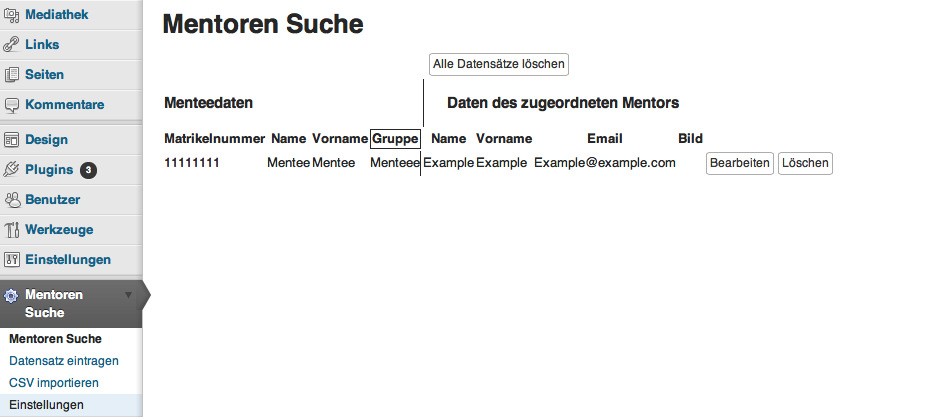
\includegraphics[angle={360}, scale=0.50]{pictures/mentsuchergmenue.png}
	    \caption{Ausgabe Top-Level-Menü-Funktion}
	    \label{img:ausgtlmfunk}
	    	\end{center}
   \end{figure}
\subsection{Erstellen von Submenüs}\label{erstum}
Da bereits im Abschnitt \ref{ersttlm} beschrieben wurde, wie Top-Level-Menüs zu erstellen sind, wird nun auf die Submenüs - oder auch Untermenüs - eingegangen.\newline
Beispielsweise, wäre laut Williams/Richard/Tadlock\footcitetgedr[Vgl.][61]{BWPWP11}  das Menü \emph{Allgemein} im Backend von Wordpress das Submenü, während \emph{Einstellungen} das Top-Level-Menü. \newline
Um ein solches Untermenü zu erstellen, wird die Funktion \emph{add\_submenu\_page} verwendet\footcitetint[Vgl.][]{MMTFRADSUBMP13} :
\lstset{language={PHP},caption={Syntax der Submenü - Funktion},label=BSPSBMFUNWP}
\lstset{
 morekeywords={function,do_action,global,\$exit_msg}
}
\begin{lstlisting}
<?php 
...
  add_submenu_page( $parent_slug, $page_title, $menu_title, $capability, $menu_slug, $function ); 
...
?>
\end{lstlisting}
Dabei sind die Parameter wie folgt zu verstehen:
\begin{enumerate}
	\item \textbf{\$parent\_slug}
	\begin{itemize}
		\item Hierbei handelt es sich einen nicht-optionalen Parameter, welcher den Namen des Obermenüs beschreibt. Falls ein Menü geschrieben werden soll, welches keinen Menü als Unterpunkt auftaucht, kann der Wert \emph{NULL} oder \emph{options.php} gesetzt werden.
	\end{itemize}
	\item \textbf{\$page\_title}
		\begin{itemize}
		\item Der Seitentitel beschreibt den Text, der auf der Seite als Titel nach dem anklicken des Submenüs angezeigt wird. Dieser ist in Form eines Strings zu verwenden und nicht optional.
	\end{itemize}
	\item \textbf{\$menu\_title}
	\begin{itemize}
		\item Der Menütitel beschreibt den Titel, welcher in dem Untermenü-Button angezeigt wird.
	\end{itemize}
	\item \textbf{\$capability}
	\begin{itemize}
		\item  Die \$capability beschreibt die Rechtezuteilung, damit User diese sehen oder nicht sehen können: Je nachdem, wie die Rechtevergabe aussieht. Diese Angabe ist nicht optional. Dabei kann zwischen verschiedenen Hierarchien von Rechten unterschieden werden. Diese fangen an oberster Stelle mit dem Super-Administrator und Administrator an, und hören bei dem Abbonennten auf. Weitere Informationen finden sich unter \url{http://codex.wordpress.org/Roles\_and\_Capabilities}.
	\end{itemize}
	\item \textbf{\$menu\_slug}
	\begin{itemize}
		\item  Dies ist Parameter, um das Menü eindeutig anzusprechen. Dies ist erforderlich, um das Elternmenü nicht mehrmals zu erstellen. Diese Angabe ist erforderlich.
	\end{itemize}
	\item \textbf{\$function}
	\begin{itemize}
		\item Hierbei handelt es sich um einen String in Form einer Funktion, welcher als Ausgabe für die angeklickte Seite dient. Dieser ist optional.
	\end{itemize}
\end{enumerate}
Die Theorie wird nun anhand eines Beispiels im Abschnitt \ref{bsperstum} erläutert.
\subsubsection{Beispiel Untermenü aus Mentoren-Suche}\label{bsperstum}
Die bereits genannten Parameter sollen nun anhand von einem Beispiel aus der Mentoren-Suche veranschaulicht werden. \newline
\lstset{language={PHP},caption={Beispiel Mentoren-Suche Submenü},label=BSPSUBMENUE}
\lstset{
 morekeywords={function,do_action,global,\$exit_msg}
}
\begin{lstlisting}
<?php 
...
function me_dataset_import() {
	add_submenu_page( 'mentees', __('Datensatz eintragen','mentoren-suche'), __('Datensatz eintragen','mentoren-suche'), 'unfiltered_html', 'row-import', 'ms_row_new');
}
...
?>
\end{lstlisting}
Die Funktion \emph{me\_dataset\_import} ist dafür da, den Untermenüpunkt \emph{Datensatz eintragen} in das Menü \emph{Mentoren Suche} einzubinden. Anschließend wird dann die Funktion \emph{row\_import}, welche dann die Funktion \emph{ms\_row\_new} aufruft. Diese ist zum Eintragen von Datensätzen vorhanden. Abschließend ist dieses Beispielmenü in der Abbildung \ref{img:aussub} dargestellt.
\newpage
  \begin{figure}[htbp]
	\begin{center}
		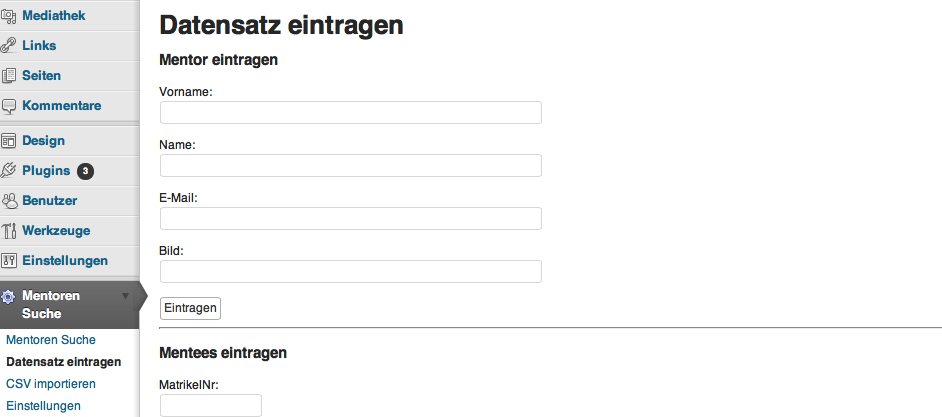
\includegraphics[angle={360}, scale=0.4]{pictures/mentsuchergsubmenue.png}
	    \caption{Ausgabe Submenü-Funktion}
	    \label{img:aussub}
	    	\end{center}
   \end{figure}
Im nächsten Kapitel geht es nicht um das neue anlegen von Top- oder Submenüs, sondern um die Integration von Menüs in bereits bestehende Standard-Menüs von Wordpress.
\subsection{Integration in bestehende Menüs}\label{integration}
Nachdem bereits erwähnt wurde, wie Top-Level- und Submenüs erstellt werden, kommt nun zum Schluss die Integration von Einstellungsseiten in eine vorhandene Menüstruktur.\newline
Wenn ein Plugin einen überschaubaren Umfang hat, besitzt es meistens auch nicht mehr als eine Einstellungsseite. Nun könnte ein Programmierer auch für diese Seite ein einzelnes Top-Level- und/oder Submenü erstellen. Alternativ dazu gibt es laut Williams/Richard/Tadlock\footcitetgedr[Vgl.][Seite 62]{BWPWP11} die Möglichkeit, bereits in vorhandenen Menüstrukturen, Untermenüs zu erstellen. Dies könnte je nach Kontext des Plugins beispielsweise unter Design oder Einstellungen eingebaut werden. Weitere Beispiele sind der Abbildung \ref{img:UEADWP} gezeigt.
  \begin{figure}[htbp]
	\begin{center}
		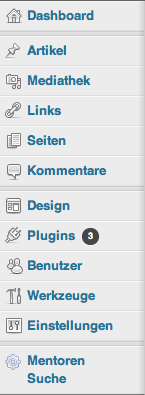
\includegraphics[angle={360}, scale=0.48]{pictures/dash.png}
	    \caption{Übersicht Admin-Bereich von Wordpress}
	    \label{img:UEADWP}
	    	\end{center}
   \end{figure}
\newpage Es gibt unter Wordpress sehr viele verschiedene Möglichkeiten, um die Standardmenüs mit eigenen zu erweitern. An dieser Stelle wird die Funktion \emph{add\_options\_page} verwendet. Die allgemeine Syntax sieht folgendermaßen aus\footcitetint[Vgl.][]{MMTADOPPA13}:
\lstset{language={PHP},caption={Syntax zum integrieren von Menüs in bereits vorhandene},label=BSPINTMENVOR}
\lstset{
 morekeywords={function,do_action,global,\$exit_msg}
}
\begin{lstlisting}
<?php
add_options_page( $page_title, $menu_title, $capability, $menu_slug, $function);
?> 
\end{lstlisting}
Im weiteren werden nun die einzelnen Parameter laut Wordpress Codex erläutert:
\begin{enumerate}
	\item \textbf{\$page\_title}
	\begin{itemize}
		\item Hierbei handelt es sich um einen Parameter vom Typ String und beschreibt den Titel der Seite, die beim auswählen des Menüs geöffnet wird. Diese Angabe nicht erforderlich.
	\end{itemize}
	\item \textbf{\$menu\_title}
		\begin{itemize}
		\item Auch dieser Parameter ist nicht optional und beschreibt den dargestellten Text für das Menü - also die Menübezeichnung. 
	\end{itemize}
	\item \textbf{\$capability}
	\begin{itemize}
		\item Der zweite Parameter beschreibt die Mindestfähigkeit an Rechten, um das Untermenü anklicken zu können. Auch hierbei handelt es sich im eine Rechte-Hierarchie, welche genauer unter der folgenden Adresse tiefer beschrieben wird: \url{http://codex.wordpress.org/Roles\_and\_Capabilities}.
	\end{itemize}
	\item \textbf{\$menu\_slug}
	\begin{itemize}
		\item  Hierbei handelt es sich um einen eindeutigen Indentifizierer, um das Untermenü eindeutig zu beschreiben. Auch dieser Parameter ist nicht optional.
	\end{itemize}
	\item \textbf{\$function}
	\begin{itemize}
		\item Hingegen den anderen Parametern, ist dieser Paramter optional und beschreibt eine Funktion, die aufgerufen wird, um den Inhalt der aufgerufenen Seite darzustellen.
	\end{itemize}
\end{enumerate}
Soweit an dieser Stelle zur Theorie. Im nächsten Unterabschnitt wird dann ein Beispiel gezeigt und erläutert.
\subsubsection{Beispiel Integration von Submenüs}
In diesem Beispiel, welches in Listing \ref{BSPHINUMVM} dargestellt ist, wird unter den Einstellungen im Dashboard von Wordpress ein weiteres Untermenü eingefügt.\footcitetgedr[Vgl.][Seite 62 - 63]{BWPWP11}
\lstset{language={PHP},caption={Beispiel hinzufügen eines Untermenüs zu vorhandenen Menüs},label=BSPHINUMVM}
\lstset{
 morekeywords={function,do_action,global,\$exit_msg}
}
\begin{lstlisting}
<?php
...
add_action( 'admin_menu', 'boj_menuexample_create_menu' );

function boj_menuexample_create_menu() {
	//create a submenu under Settings
	add_options_page( 'My Plugin Settings Page', 'Menu 	Example Settings', 'manage_options', __FILE__, 'boj_menuexample_settings_page' );
	}
...
<?
\end{lstlisting}
In diesem Beispiel wird ein Untermenü mit dem Namen \emph{My Plugin Settings Page} im Einstellungsmenü dargestellt (siehe Zeile 7). Anschließend wird der Seitentitel auch auf \emph{My Plugin Settings Page} gesetzt und die Mindestfähigkeit an Rechten auf manage\_options gesetzt (was soviel bedeutet, dass der Benutzer die Rechte haben muss, um die Einstellungen zu verändern / auf dieses Menü zugreifen zu können). Abschließend wird dann eine Funktion genannt, welche bei Aufruf des Menüs ausgeführt werden muss.\newline
Schlussendlich sieht dies dann folgendermaßen aus (siehe Abbildung \ref{img:untermenuinvorhmenu}):
  \begin{figure}[htbp]
	\begin{center}
		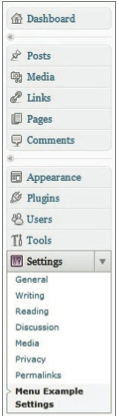
\includegraphics[angle={360}, scale=0.61]{pictures/untermenuinvorhmenu.png}
	    \caption{Eigenes Untermenü in vorhandene Menüstrukturen eingebunden}
	    \label{img:untermenuinvorhmenu}
	    	\end{center}
   \end{figure} \newline
Weitere Möglichkeiten, um Submenüs in Wordpress einzubinden sind beispielsweise\footcitetgedr[Vgl.][Seite 63]{BWPWP11}
\begin{enumerate}
\item add\_dashboard\_page - Fügt ein Untermenü zum Dashboard hinzu
\item add\_theme\_page - Fügt ein Untermenü zum Thememenü hinzu
\item add\_plugins\_page - Fügt ein Untermenü zum Pluginmenü hinzu
\end{enumerate}
Weitere sind unter der folgenden Adresse zu finden:\url{http://codex.wordpress.org/Administration\_Menus#Admin\_Menu\_Functions}\newline
Die Autoren Williams/Richard/Tadlock\footcitetgedr[Vgl.][Seite 63]{BWPWP11} raten an dieser Stelle dazu, wenn ein Plugin nur eine einzelne Einstellungsseite hat, diese als Untermenü in ein vorhandenes einzubinden. Wenn allerdings mehr als eines (wie beispielsweise bei der Mentoren-Suche der Fall), sollte ein eigenes erstellt werden.
\subsection{Ausblick} 
Insgesamt gibt es mehrere Möglichkeiten - je nach Bedarf - ein Menü neu anzulegen oder zu integrieren. \newline
Es sollte allerdings darauf geachtet werden, dass bei einer möglichen Veröffentlichung des Plugins auch in die Dokumentation gehört, wo die Plugineinstellungen gefunden werden können. Dies ist vor allem von großen Interesse, wenn neue Menüs in bestehende integriert werden.\footcitetgedr[Vgl.][Seite 60 - 61]{BWPWP11}
Weitere Informationen zu diesem Thema finden sich unter:
\begin{enumerate}
	\item \url{http://codex.wordpress.org/Function\_Reference} 	\item \url{http://codex.wordpress.org/Administration\_Menus}
	\item	\url{http://codex.wordpress.org/User\_Levels}
\end{enumerate}